\documentclass[../main/main.tex]{subfiles}
\begin{document}

\section{Schemat konstrukcji mechanicznej}
Sklejka, dykta, trytki, klej.

\section{Schemat elektroniczny}

Poniżej zamieszczono schemat połączeń.

\begin{figure}[h]
\centering
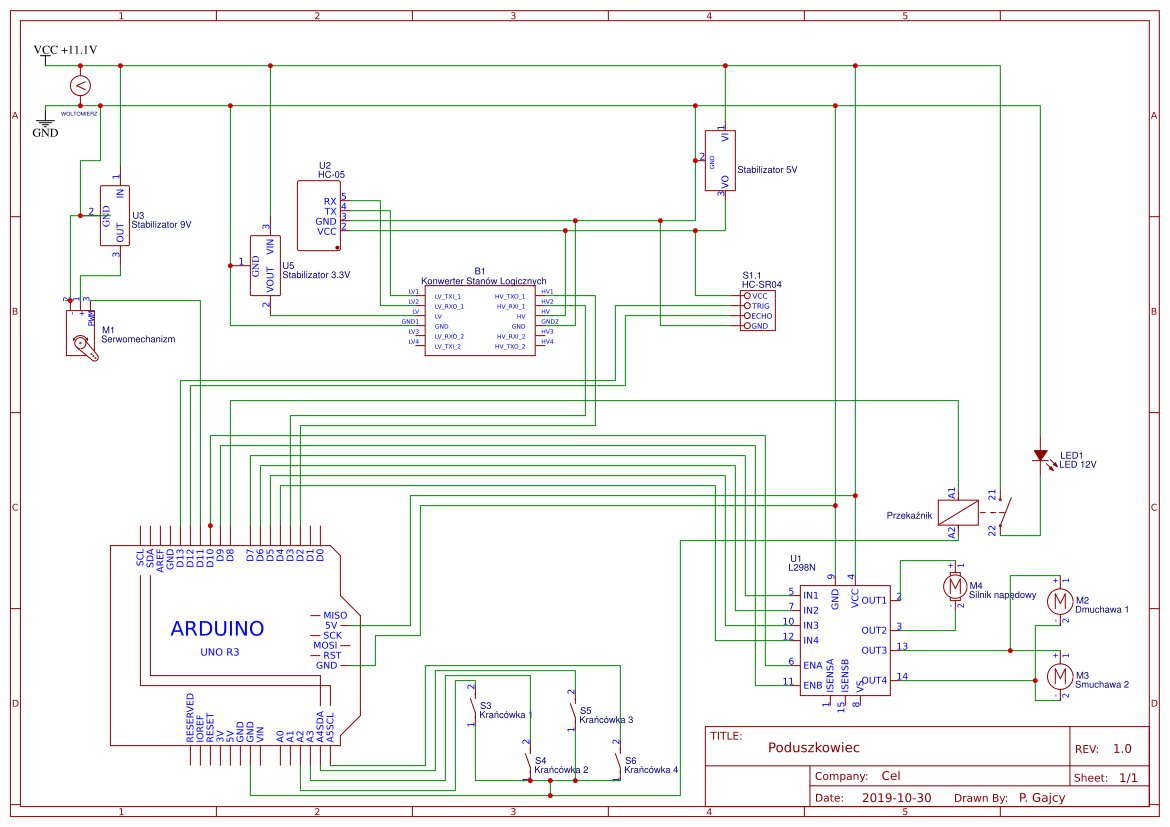
\includegraphics[width=1\textwidth]{../obrazy/schemat_aktualny.png}
\caption{Wstępny schemat}
\label{schemat_ogólny}
\end{figure}

Tekst można zamknąć w pudełku: \fbox{o tak}.

\section{Komponenty}
Spis urządzeń i podzespołów wraz z opisem.

\subsection{Napęd}
Dmuchawy i silnik napędowy.

\subsection{Ster kierunku}
Serwomechanizm.

\subsection{Sterownik silników}
L298N

\subsection{Mikrokontroler}
Arduino

\subsection{moduł Bluetooth}
HC-05

\subsection{Czujnik odległości}
HC-SR04

\subsection{Detekcja przeszkód}
Krańcówki

\subsection{Inne}
\subsubsection{LED}
Oświetlenie wraz z przekaźnikiem.

\subsubsection{Konwerter 5V-3.3V}
Konwersja stanów logicznych.

\subsection{Zasilanie}
Trzy linie zasilania.

\section{Montaż konstrukcji mechanicznej}
Deski i śrubki.

\section{Montaż podzespołów elektronicznych}
Przebieg
\subsubsection{Prototyp}
NA pająka.
\subsubsection{Płytka PCB}
Pożadniej

\section{Gotowy model}

\end{document}

  
